%% This is file `elsarticle-template-1-num.tex',
%%
%% Copyright 2009 Elsevier Ltd
%%
%% This file is part of the 'Elsarticle Bundle'.
%% ---------------------------------------------
%%
%% It may be distributed under the conditions of the LaTeX Project Public
%% License, either version 1.2 of this license or (at your option) any
%% later version.  The latest version of this license is in
%%    http://www.latex-project.org/lppl.txt
%% and version 1.2 or later is part of all distributions of LaTeX
%% version 1999/12/01 or later.
%%
%% The list of all files belonging to the 'Elsarticle Bundle' is
%% given in the file `manifest.txt'.
%%
%% Template article for Elsevier's document class `elsarticle'
%% with numbered style bibliographic references
%%
%% $Id: elsarticle-template-1-num.tex 149 2009-10-08 05:01:15Z rishi $
%% $URL: http://lenova.river-valley.com/svn/elsbst/trunk/elsarticle-template-1-num.tex $
%%
\documentclass[preprint,12pt]{elsarticle}

%% Use the option review to obtain double line spacing
%% \documentclass[preprint,review,12pt]{elsarticle}

%% Use the options 1p,twocolumn; 3p; 3p,twocolumn; 5p; or 5p,twocolumn
%% for a journal layout:
%%\documentclass[final,1p,times]{elsarticle}
%% \documentclass[final,1p,times,twocolumn]{elsarticle}
%% \documentclass[final,3p,times]{elsarticle}
%% \documentclass[final,3p,times,twocolumn]{elsarticle}
%% \documentclass[final,5p,times]{elsarticle}
%% \documentclass[final,5p,times,twocolumn]{elsarticle}

%% if you use PostScript figures in your article
%% use the graphics package for simple commands
%% \usepackage{graphics}
%% or use the graphicx package for more complicated commands
\usepackage{graphicx}
%% or use the epsfig package if you prefer to use the old commands
%% \usepackage{epsfig}

%% The amssymb package provides various useful mathematical symbols
\usepackage{amssymb}
%% The amsthm package provides extended theorem environments
%% \usepackage{amsthm}

%% The lineno packages adds line numbers. Start line numbering with
%% \begin{linenumbers}, end it with \end{linenumbers}. Or switch it on
%% for the whole article with \linenumbers after \end{frontmatter}.
%% \usepackage{lineno}

%% natbib.sty is loaded by default. However, natbib options can be
%% provided with \biboptions{...} command. Following options are
%% valid:

%%   round  -  round parentheses are used (default)
%%   square -  square brackets are used   [option]
%%   curly  -  curly braces are used      {option}
%%   angle  -  angle brackets are used    <option>
%%   semicolon  -  multiple citations separated by semi-colon
%%   colon  - same as semicolon, an earlier confusion
%%   comma  -  separated by comma
%%   numbers-  selects numerical citations
%%   super  -  numerical citations as superscripts
%%   sort   -  sorts multiple citations according to order in ref. list
%%   sort&compress   -  like sort, but also compresses numerical citations
%%   compress - compresses without sorting
%%
%% \biboptions{comma,round}

% \biboptions{}


\journal{Nuclear Physics B}

\begin{document}

\begin{frontmatter}

%% Title, authors and addresses

%% use the tnoteref command within \title for footnotes;
%% use the tnotetext command for the associated footnote;
%% use the fnref command within \author or \address for footnotes;
%% use the fntext command for the associated footnote;
%% use the corref command within \author for corresponding author footnotes;
%% use the cortext command for the associated footnote;
%% use the ead command for the email address,
%% and the form \ead[url] for the home page:
%%
%% \title{Title\tnoteref{label1}}
%% \tnotetext[label1]{}
%% \author{Name\corref{cor1}\fnref{label2}}
%% \ead{email address}
%% \ead[url]{home page}
%% \fntext[label2]{}
%% \cortext[cor1]{}
%% \address{Address\fnref{label3}}
%% \fntext[label3]{}

\title{Semiconductor phonon and charge transport Monte Carlo simulation using Geant4}

%% use optional labels to link authors explicitly to addresses:
%% \author[label1,label2]{<author name>}
%% \address[label1]{<address>}
%% \address[label2]{<address>}

\author{}

\address{}

\begin{abstract}

A phonon and charge transport simulation based on the Geant4 Monte Carlo toolkit is presented. The transport code is capable of propagating acoustic phonons as well as electrons and holes in cryogenic crystals. Anisotropic phonon propagation, oblique carrier propagation and phonon emission by accelerated carriers are all taken into account. The simulation is successfull in reproducing theoretical predictions and experiemtntal observations sch as phonon caustics, heat pulse propagation times and mean carrier drift velocities.

Implementation of the transport code using the Gent4 toolkit ensures availability of the transport code to the wider scientific community.

\end{abstract}

\begin{keyword}
%% keywords here, in the form: keyword \sep keyword

%% MSC codes here, in the form: \MSC code \sep code
%% or \MSC[2008] code \sep code (2000 is the default)

\end{keyword}

\end{frontmatter}

%%
%% Start line numbering here if you want
%%
%% \linenumbers


%% The Appendices part is started with the command \appendix;
%% appendix sections are then done as normal sections
%% \appendix

%% \section{}
%% \label{}

\section{Introduction}
\label{sec:Introduction}

In this paper we present a Monte Carlo simulation of phonon and charge transport in Semiconductor crystals using Geant4. Geant4 is a sophisticated C++ based Monte Carlo simulation toolkit maintained by an international collaboration and freely available under an open source license \cite{Geant-A} \cite{Geant-B}. The toolkit was originally developed in support of High Energy Physics (HEP) experiments. It provides functionality for the simulation of the passage of particles through complex geometries and aims to accurately simulate all interactions of the particles with the matter through which they pass. Today, the Geant4 toolkit is an important tool both for HEP particle accelerator based experiments building Detector Monte Carlo(DMC) simulations as well as experiments wishing to estimate backgrounds from environmental or cosmic ray radiation sources [cite]\cite{Brandt}.

In it's current incarnation, the Geant4 toolkit is entirely focused on free particles and does not take into account crystal physics and conduction/valence band interactions of the low energy charge carriers and phonons relevant to condensed matter physics. This paper documents our effort to build a cohesive Geant4 Condensed Matter Physics Monte Carlo simulation toolkit, G4CMP. This effort is motivated by the Cryogenic Dark Matter Search (CDMS) dark  matter direct detection experiment \cite{CDMS-A}\cite{CDMS-B}\cite{CDMS-C}. The CDMS detectors are cylindrical Germanium crystals of approximate size $75$mm $\times$ $25$mm [cite], cooled to ~$60$mK. Dark matter particles may recoil from Ge nuclei via the weak force and thus create phonons and free electron-hole pairs within the crystal [Lindhardt]. Electron-hole pairs are collected at the crystal surface by a small (~V/cm) drift field. Phonons are detected by Transition Edge Sensor (TES) bolometers. The need for an accurate Detector MonteCarlo simulation of the CDMS detector has provided the chief motivation for the work described in this paper.

The phonon and charge transport code described here attempts to accurately model all physics processes believed to be relevant to phonon and charge collection at cryogenic temperatures. This includes anisotropic phonon transport/phonon focusing, phonon isotope scattering, anharmonic downconversion, oblique carrier propagation and emission of Luke-Neganov phonons by accelerated carriers. We believe that the resulting G4CMP framework is sufficiently general that it can be useful to other experiments employing cryogenically cold charge or phonon detectors. 

\section{Phonon Transport}
\label{sec:PhononTransport}

Phonon transport was the first component of the G4CMP framework to be developed and early results were presented at LTD-14 \cite{Brandt}. Since the phonon transport code described here is intended for temperatures $T<1$K, scattering off thermally excited background phonons is ignored. Currenly, only acoustic phonons are simulated.

\subsection{Anisotropic transport and phonon focusing}
\label{sec:Focusing}

Phonons are quantized vibrations of the crystal lattice. The propagation of phonons is governed by the three-dimensional wave equation \cite{Wolfe}:

\begin{equation}
\label{eq:3DWave}
\rho \omega ^2e_i=C_{ijlm}k_jk_me_l
\end{equation}

where $\rho$ is the crystal mass density, $\omega$ is the phonon frequency, $\vec{e}$ is the polarization vector, $\vec{k}$ is the wave vector and $\vec{C}_{ijml}$ is the elasticity tensor.

For any given wave vector $\vec{k}$ Equation \ref{eq:3DWave} has three eigenvalues $\omega$ and three eigenvectors $\vec{e}$. These correspond to the three different polarization states \textit{Fast Transverse (FT), Slow Transverse (ST)} and \textit{Longitudinal (L)}. The actual direction and velocity of propagation of phonons is given by the group velocity vector $\vec{v_g} = d\omega/dk$. The group velocity can be calculated by interpreting $\omega$ in Equation \ref{eq:3DWave} as a function of $\vec{k}$:

\begin{equation}
\label{eq:GroupV}
\vec{v_g}=\frac{d \omega (\vec{k})}{d\vec{k}}=\nabla_k \omega (\vec{k})
\end{equation}

Due to the anisotropy in $C_{ijlm}$, Eq. \ref{eq:GroupV} yields a group velocity $\vec{v_g}$ which is not parallel to the phonon momentum $\hbar\vec{k}$. Instead, phonons are focused onto propagation directions which correspond to the highest density of eigenvectors $\vec{k}$. This focusing gives rise to caustics when observing the energy  distribution resulting from a point-like phonon source isotropic in $\vec{k}$-space. The resulting caustics can be observed using microcalorimeters \cite{Nothrop}. It can be seen from Figure\ref{fig:caustics}. that the caustics simulated by the Geant4 phonon transport code are in good agreement with experimental observations. 

For the purposes of the G4CMP phonon transport code, the wave eqaution is not solved in real time but rather a look-up table is generated which maps $\vec{k}$ onto $\vec{v_g}$. Bilinear interpolation is used to generate a continuous mapping function. Phonon focusing and methods for solving the three-dimensional wave equations are treated in great detail in the book by Wolfe \cite{Wolfe}.

Also consider \ref{fig:caustics}.

\begin{figure}
	\centering
		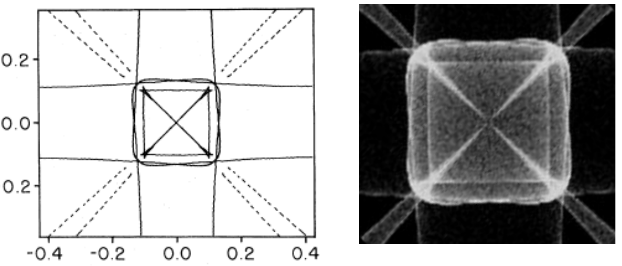
\includegraphics[width=1.00\textwidth]{caustics.png}
	\caption{\textbf{Left:} outline of phonon caustics in Germanium as predicted by Nothrop and Wolfe \cite{Nothrop}. \textbf{Right:} Phonon caustics as simulated using the Geant4 phonon transport code. This results is in good agreement with both the theoretical prediction and experimental observations reported by Nothrop and Wolfe \cite{Nothrop} }
	\label{fig:caustics}
\end{figure}

\subsection{Phonon processes}
\label{sec:Processes}

In addition to the phonon equation of motion, which is given by the three dimensional wave equation Eq.\ref{eq:3DWave}, two processes are relevant to acoustic phonon transport in cryogenic crystals: Isotope scattering and anharmonic down conversion[cite]. The scattering and downconversion rates for phonons in the cryogenic crystal are given by \cite{Tamura2}:

\begin{equation}
\label{eq:ScatterRate}
\Gamma_{scatter} = B\nu^4
\end{equation}

\begin{equation}
\label{eq:anhRate}
\Gamma_{anh} = A\nu^5
\end{equation}

where $\Gamma_{scatter}$ is the number of scattering events per unit time, $\Gamma_{anh}$ is the number of anharmonic downconversion events per unit time, $nu$ is the phonon frequency and $A$, $B$ are constants of proportionality derived from the elasticity tensor. There value for Germanium has been discussed in an earlier paper \cite{Brandt} and methods for their derivation can be found in the literature \cite{Tamura1} \cite{Tamura2}.

The isotope scattering process occurs when a phonon interacts with an isotopic substitution site in the lattice. It is effectively an elastic scattering process during which we assume the phonon momentum vector to be randomized. During this scattering process the phonon polarization state can change freely between the three states $L$, $ST$, $FT$. The branching ratio between the three polarizations is determined by the relative density of allowed states for each polarization.This change between polarization states is often referred to as mode mixing.

The anharmonic down conversion process causes a single energetic phonon to decay into two phonons of reduced energy. In the smulation, this process conserves energy but not momentum, since momentum is exchanged with the crystal lattice. While in theory all three polarization states can decay, the downconversion rate of $L$-phonons completely dominates the energy evolution of the phonon system, with downconversion events from other polarization states being negligigible \cite{Tamura2}.


As can be seen from eqs. \ref{eq:ScatterRate} \ref{eq:anhRate}, both process rates strongly depend on phonon energy $\hbar \nu$. High energy phonons ($\nu$ of order THz)start out in a diffusive regime with high isotope scattering and downconversion rates and mean free paths of order microns. Once a few downconversion events have occured, phonon mean free paths increase to be of order the size of a typical rare event search crystal detector (of order $0.1$ m linear dimension). This transition from a diffuse to a ballistic transport mode is commonly referred to as ``quasi-diffuse'' and it controls the time evolution of phonon heat pulses. Simulation of heat pulse propagation using our Geant4 transport code has been described previously \cite{Brandt} and shows good agreement with experiment.

Anharmonic downconversion and isotope scattering are well understood and are discussed in great detail in the literature \cite{Tamura1}\cite{Tamura2}\cite{Wolfe}\cite{Tamura3}.




\section{Charge Transport}
\label{sec:ChareTransport}


\section{Conclusion}
\label{sec:Conclusion}



%% References
%%
%% Following citation commands can be used in the body text:
%% Usage of \cite is as follows:
%%   \cite{key}          ==>>  [#]
%%   \cite[chap. 2]{key} ==>>  [#, chap. 2]
%%   \citet{key}         ==>>  Author [#]

%% References with bibTeX database:

\bibliographystyle{model1-num-names}
\begin{thebibliography}{99}


\bibitem{Geant-A}
J. Allison et al., {\it IEEE Transactions on Nuclear Science} \textbf{53}, 270 - 278, (2006).

\bibitem{Geant-B}
S. Agostinelli et al., {\it Nuclear Instruments and Methods A} \textbf{506}, 250 - 303, (2003).

\bibitem{Brandt}
D. Brandt et al., {\it Journal of Low Temperature Physics} \textbf{167}, 485 - 490, (2011).

%\bibitem{Enss}
%C. Enss, {\it Cryogenic Particle Detection },Springer Verlag, Germany (2005)

\bibitem{CDMS-A}
Z. Ahmed et al., {\it Science} \textbf{327}, 1619, (2010).

\bibitem{CDMS-B}
Z. Ahmed et al., {\it Phys. Rev. D} \textbf{84}, 011102, (2011).

\bibitem{CDMS-C}
C. Collaboration et al., {\it arxiv astro-ph.CO} \textbf{1304.4279},(2013)

%\bibitem{Sanglard}
%V. Sanglard et al., {\it Phys. Rev. D.} \textbf{71}, 122002, (2005).

%\bibitem{Lang} %CRESST
%Rafael F. Lang and Wolfgang Seidel, {\it N. J. Phys} \textbf{11}, 105017, (2009).

%\bibitem{Arnaboldi}%CUORE
%C. Arnaboldi et al., {\it NIM A} \textbf{3}, 775, (2004).


\bibitem{Brink}
P. Brink et al., {\it NIM A} \textbf{2}, 414, (2006)

%\bibitem{Hurley}
%D.C. Hurley and J.P. Wolfe, {\it Phys. Rev. B} \textbf{32}, 2568, (1985)

\bibitem{Nothrop}
G.A. Nothrop and J.P. Wolfe, {\it Phys. Rev. Lett.} \textbf{19}, 1424, (1979)

\bibitem{Tamura1}
S. Tamura, {\it J. Lo. T. Phys.} \textbf{93}, 433, (1993)

\bibitem{Tamura2}
S. Tamura, {\it Phys. Rev. B.} \textbf{48}, 13502, (1993)

\bibitem{geant}
J. Allison et al., {\it IEEE Trans. Nucl. Sci.} \textbf{1}, 270, (2006)


\bibitem{Wolfe}
J.P. Wolfe, {\it Imaging Phonons, Chapter 2},42, Cambridge University Press, United Kingdom (1998) 

\bibitem{Tamura3}
S. Tamura,{\it Phys. Rev. B.} \textbf{31}, (1985)

%\bibitem{Leman}
%S.W. Leman et al., {\it These procedings},(2011)

%\bibitem{McCarthy}
%K.A. McCarthy et al., {\it These procedings},(2011)

%\bibitem{Anderson}
%A. Anderson et al., {\it These procedings},(2011)


\end{thebibliography}

%% Authors are advised to submit their bibtex database files. They are
%% requested to list a bibtex style file in the manuscript if they do
%% not want to use model1-num-names.bst.

%% References without bibTeX database:

% \begin{thebibliography}{00}

%% \bibitem must have the following form:
%%   \bibitem{key}...
%%

% \bibitem{}

% \end{thebibliography}


\end{document}

%%
%% End of file `elsarticle-template-1-num.tex'.
